\section{Example of transducer for approximate Kleenex program}
\label{app:approx-kleenex-example}

\begin{figure}[!ht]
  \begin{subfigure}[t]{1\textwidth}
    \centering
    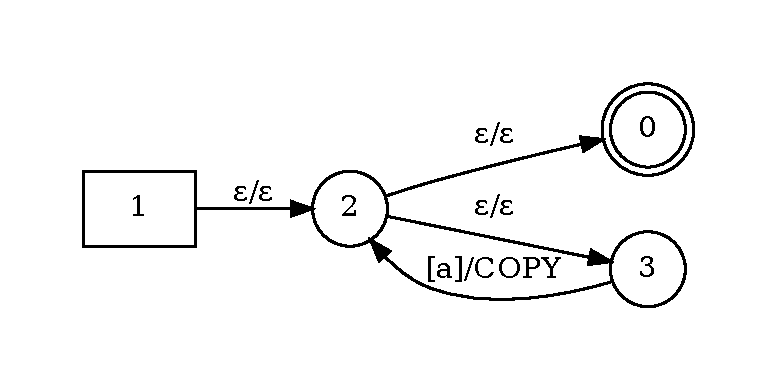
\includegraphics[width=0.5\textwidth]{images/as_exact.pdf}
    \caption{Transducer for the original program.}
  \end{subfigure}
  ~
  \noindent\makebox[\textwidth]{%
  \begin{subfigure}[t]{1.4\textwidth}
    \centering
    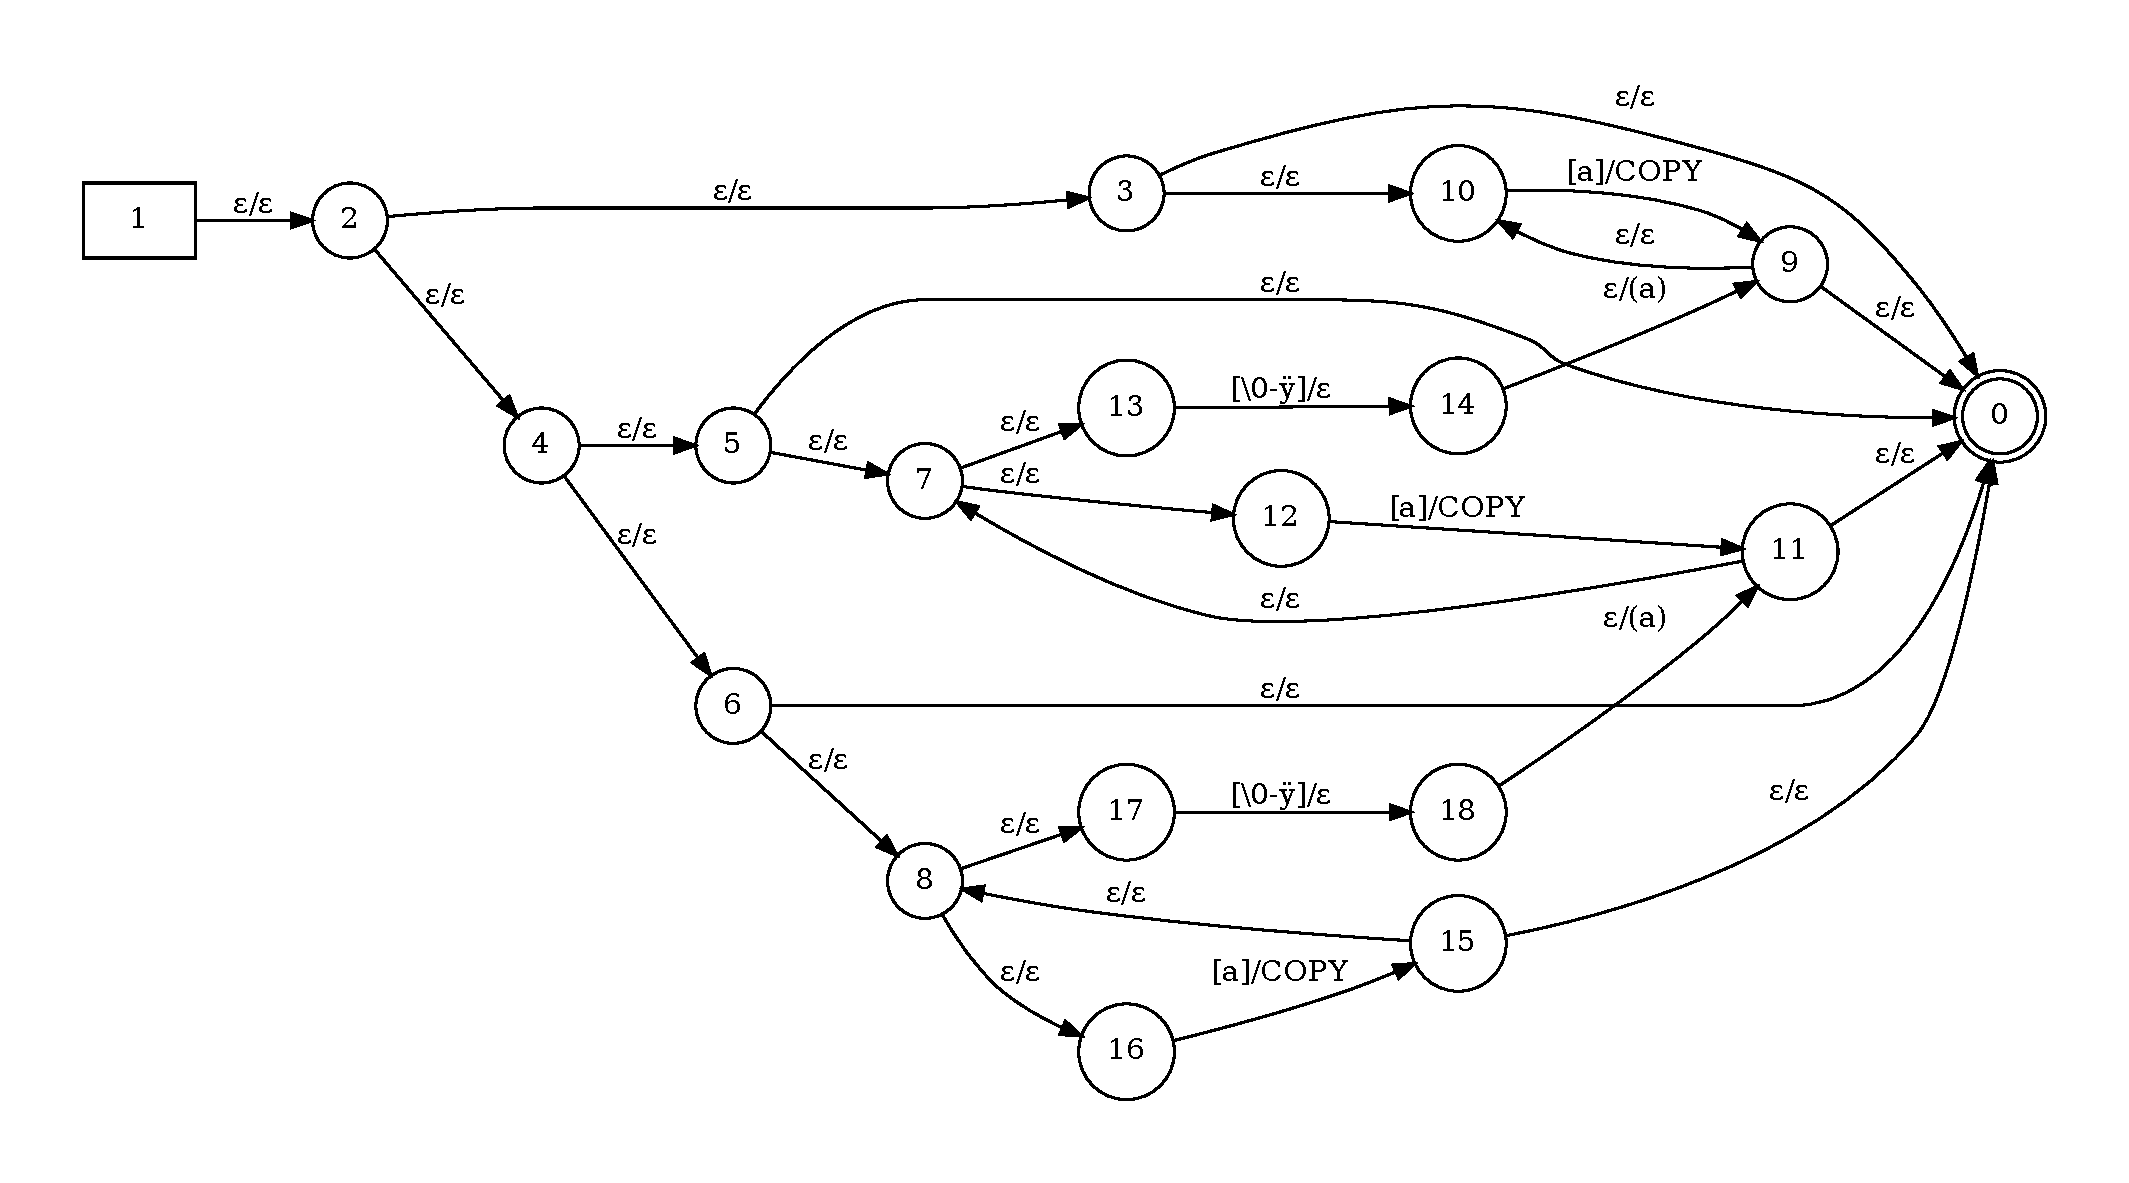
\includegraphics[width=\textwidth]{images/as_k2_hamming.pdf}
    \caption{Transducer for the rewritten program.}
  \end{subfigure}}
  \caption{Visualization of transducers for the original Kleenex program
    accepting exactly $a^*$ and the rewritten program accepting $a^*$ with
    $k=2$ errors using Hamming distance.}
\end{figure}

%%% Local Variables:
%%% mode: latex
%%% TeX-master: "main"
%%% End:
